\chapter{Control Architecture}
\section{Introduction}
Vukobratovic \cite{Vuk1970} was one of the first researchers involved in the stability of bipedal robots, followed by \cite{Kaj2001} and \cite{Kim2004}. In all their studies, the biped robot was usually represented by a planar inverted pendulum with the base representing the foot and the ankle joint. And in the latest control strategies, researchers divide robot balance control into the hip strategy and the ankle strategy \textcolor{red}{REFERENCIA Y EXTENDER MÁS}. The basis of both stategies are close to the ZMP areas explained in previous sections. When the robot is in a stable posture and a disturbance is applied, depending the magnitude or the application point of that distrubance, the robot will react different. If the change of the ZMP position remains in a stable area, the control will react by the motion of the ankle joints to recover the robot balance. Nevertheless, if the ZMP position reaches an uncertain-stability area, it will be also necessary to move the hip joints to recover balance. Even a gait will be necessary if the loss of stability is unavoidable. 

A humanoid is an electromechanical system, so it should have all type of errors: structure flexion, small blacklash between motion parts, etc. Also it will operate in a co-existing environment with humans, so the disturbances are unexpected at any time. Therefore, the Stabilizer is an essential element to provide stable human-like walking of a humanoid robot. The Stabilizer should perform two basic operations:
\begin{itemize}
\item[1.] When the humanoid robot walks, it should correct the robot’s walking trajectory in order to provide the secure position at any time of its motion.
\item[2.] When the humanoid robot has stopped, it should control its posture.
\end{itemize}

Thus, the Stabilizer can be decoupled into ZMP and Attitude controllers. This Master Thesis will deal with the issue of maintaining an upright posture while the robot is in a static position, without following a motion pattern.


\section{Single Inverted Pendulum Model}
The simple inverted pendulum is the most basic model used to simplify humanoids' body. The basis of the pendulum are a mass $m$ linked to a pivot point $0$ by means of a massless link of longitude $l$ as in Figure \ref{fig:pendulo_inv}.

The mass $m$ represents the total mass of the modelled system, a humanoid robot in this case, located at its Centre of Mass (CoM), and the longitude $l$ is the distance between the pivot point to the CoM. Its dynamical model in a planar, for example XZ case, is expressed by the equation \eqref{eq:pendulo}, if gravitational force is considered the only force acting in the system.

\begin{figure}
\centering
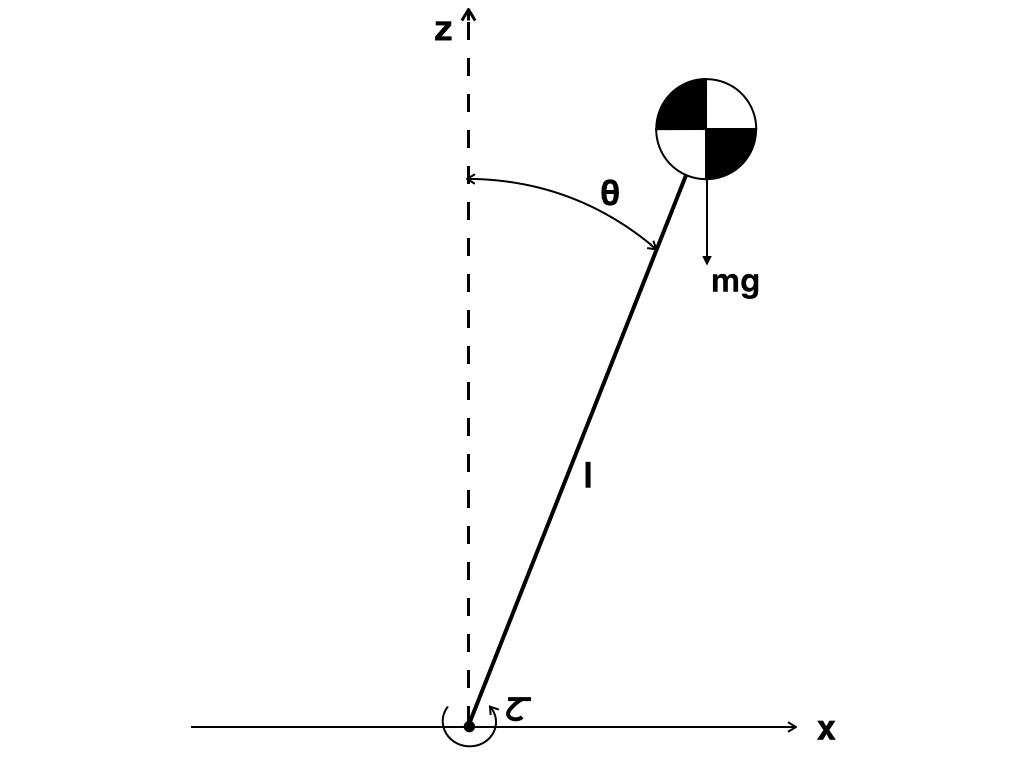
\includegraphics[scale=0.25]{pendulo_inv.png}
\caption{Single inverted pendulum.}
\label{fig:pendulo_inv}
\end{figure}

\begin{equation}
\tau_0 = ml^2 \ddot{\theta} - mgl\sin\theta
\label{eq:pendulo}
\end{equation}

where $\tau_0$ is the torque generated by the ankle joint, $\theta$ its angular position, $\ddot{\theta}$ its angular acceleration and $l$, the distance between the joint and the CoM. For simplification of a control task, let us make a linearization of nonlinear differential equations, taking the aproximation that perturbations are small enough to consider  $\sin\theta = \theta$. It is not defined how small these angles have to be in practice to apply the linearization assumptions, but in this case it is assume that $\theta \leq 5º$ Then, equation \eqref{eq:pendulo} changes to linearized equation \eqref{eq:pendulo2}
\begin{equation}
\tau_0 = ml^2 \ddot{\theta} - mgl\theta
\label{eq:pendulo2}
\end{equation}

The main complexity of this model is the fact that equation \eqref{eq:pendulo2} does not give the possibility of controlling the ZMP by angular position of the ankle joint. To overcome this problem, the inverted pendulum model can be slightly modified. The link of the pendulum which connects the ankle joint to the concentrated mass (CoM) is generally assumed to be rigid. However, in the real humanoid mechanism it is flexible because the leg length is relatively long and the mechanical structure suffers form flexibility and small backlashes. Because of this compliance, the humanoid robot exhibits the characteristics of a lightly damped structure \cite{Kim2004}. For example, in a static case when the ankle joint is under position control, a pushing external force can easily excite an oscillation. This oscillation exists even when the position error in every joint is zero. This phenomenon is prevalent in the fast dynamical gait; therefore it is very imortant to implement a control mechanism allowing ZMP fast correction considering the stiffness of the humanoid robot links. The most suitable model in this case will be a single mass inverted pendulum with compliant joint as shown in Figure \ref{fig:pendulo_elast}, where $u$ denotes the ankle joint reference angle and $\theta$ denotes the actual inclined angle produced by the compliance of the mechanical structure of the humanoid, $k$ denotes the stiffness of the leg and $\tau_0$ is the torque produced by the motor of the ankle joint to place the inverted pendulum into the desired angular position. Then, the torque $\tau_0$ should be expressed as:

\begin{equation}
\tau_0 = k(\theta - u)
\label{eq:pendulo3}
\end{equation}

\begin{figure}
\centering
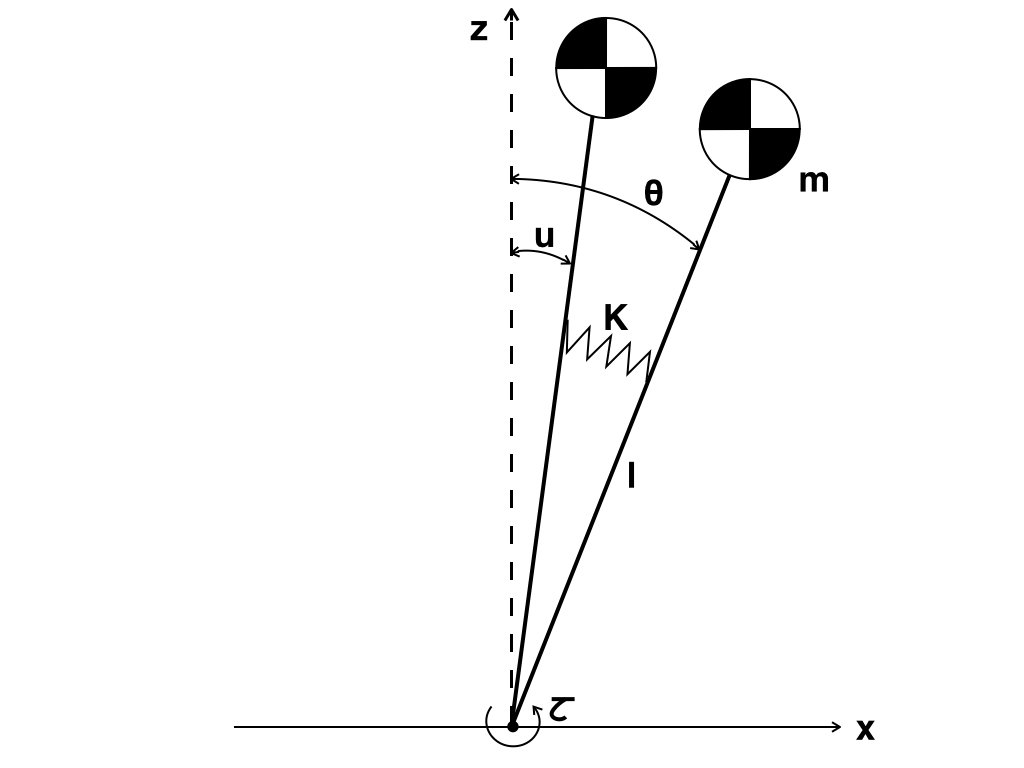
\includegraphics[scale=0.25]{pendulo_elast.png}
\caption{Single inverted pendulum with compliant joint.}
\label{fig:pendulo_elast}
\end{figure}

Taking the Laplace transform of equation \ref{eq:pendulo2}, it is obtained: 
\begin{equation}
T(s) = mgl\theta(s)- ml^2s^2\theta(s) 
\label{eq:par}
\end{equation}

The Laplace transform of equation \eqref{eq:pendulo3} is:
\begin{equation}
T(s) = k(\theta(s) - U(s))
\label{eq:par2}
\end{equation}

Reflecting $\theta(s)$ from equation \eqref{eq:par2} and placing it into the equation \eqref{eq:par} and simplifying, the transfer function is obtained:
\begin{equation}
\frac{T(s)}{U(s)} = k \frac{-s^2+(\beta - \alpha)}{s^2 + \alpha}
\label{eq:TFpar}
\end{equation}

where:
\begin{equation}
\alpha = \frac{k-mgl}{ml^2}
\end{equation}
\begin{equation}
\beta = \frac{k}{ml^2}
\end{equation}

On the other hand, from equation \textcolor{red}{[REF ECUACION zmp]} relating the moment produced by the ground reaction force around $y$ axis with $x$ ZMP direction (the planar XZ case of the inverted pendulum is considered) we can get:
\begin{equation}
\tau_y = -mgx_{ZMP} = - F_z x_{ZMP}
\label{eq:zmp}
\end{equation} 

and then the Laplace transform of the equation \eqref{eq:zmp} is:
\begin{equation}
\tau_y(s) = - F_z x_{ZMP}(s)
\label{eq:TFzmp}
\end{equation}

For the static equilibrium of the system, the moment generated y the motor of the ankle join should compensate the moment produced by the ground reaction force:
\begin{equation}
\tau_0 = \tau_y
\end{equation}

The relation between $\tau_y$ and $x_{ZMP}$ is lineal, therefore, placing \eqref{eq:TFzmp} into \eqref{eq:TFpar} we get the following transfer function relating ZMP to ankle joint position: 
\begin{equation}
\frac{x_{ZMP}(s)}{U(s)} = - k_1 \frac{-s^2+(\beta - \alpha)}{s^2 + \alpha}
\end{equation}

where $k_1 = \frac{k}{mg}$.

In the equation \eqref{eq:TFpar} $x_{ZMP}(s)$ is the output and $U(s)$ is the input of the system. It allows for the ZMP of the humanoid robot to be contolled by the position of its ankle joint. 

The state space representation of the dynamical system in the standard form is:
\begin{equation}
\mathbf{\dot{x}} = \mathbf{A}\textbf{x} + \mathbf{B}u
\label{eq:ss1}
\end{equation}

\begin{equation}
y = \mathbf{C}\textbf{x} + Du
\label{eq:ss2}
\end{equation}

where $\mathbf{x}$ is a state ($n$-vector), $y$ is the output (escalar), $u$ - control (scalar), $\mathbf{A}$ - $n \times n$ constant  matrix, $\mathbf{B}$ - $n \times 1$ constant matrix, $\mathbf{C}$ - $1 \times n$ constant matrix and $D$ a scalar.

To obtain the state representation of the inverted pendulum system let us define state variables $x_1$ and $x_2$ by:
\begin{equation}
x_1 = \theta
\label{eq:x1}
\end{equation}
\begin{equation}
x_2 = \dot{x_1} = \dot{\theta}
\label{eq:x2}
\end{equation} 

where angle $\theta$ denotes the rotation of the pendulum about the ankle and $\dot{\theta}$ its angular velocity. We consider the ZMP as the output of the system, then $y = x_{ZMP}$ in the XZ plane case. From the definition of state space equations \eqref{eq:ss1} - \eqref{eq:x2} and the linearized equations of the inverted pendulum motions \eqref{eq:pendulo2} and \eqref{eq:pendulo3} we obtain the state space representation of the system:
\begin{equation}
\begin{bmatrix}
\dot{x_1} \\
\dot{x_2}
\end{bmatrix} 
= 
\begin{bmatrix}
0 & 1 \\
-\alpha & 0
\end{bmatrix}
\begin{bmatrix}
x_1 \\
x_2
\end{bmatrix}
+
\begin{bmatrix}
0 \\
1
\end{bmatrix}
u
\label{eq:state_space}
\end{equation}
\begin{equation}
y = \begin{bmatrix}
-k_1\beta & 0 
\end{bmatrix}
\begin{bmatrix}
x_1 \\
x_2
\end{bmatrix}
+ \begin{bmatrix}
k_1
\end{bmatrix}
u
\label{eq:state_space_out}
\end{equation}

\section{Feedback in state space. The Linear Quadratic Regulator}

The quadratic optimal control method is one of the control methods applied in state space systems and it provides a systematic way of computing the state feedback control gain matrix \cite{Ogata}.
Given the state space system equation
\begin{equation}
\mathbf{\dot{x}} = \mathbf{A}\textbf{x} + \mathbf{B}\mathbf{u}
\end{equation}
the LQR determines the matrix $\mathbf{K}$ of the optimal control vector
\begin{equation}
\mathbf{u}(t) = -\mathbf{Kx}(t)
\label{eq:control}
\end{equation}
so as to minimize the performance index
\begin{equation}
J = \int_{0}^{\infty}(\mathbf{x}^{T}\mathbf{Qx}+\mathbf{u}^{T}\mathbf{Ru}) dt
\end{equation}

where $\mathbf{Q}$ is a positive-definite (or positive-semidefinite) Hermitian or real symmetric matrix and $\mathbf{R}$ is a positive-definite Hermitian or real symmetric matrix. Note that the matrices $\mathbf{Q}$ and $\mathbf{R}$ determine the relative importance of the error and the expenditure of the energy of the control signals.
The linear control law given by equation \eqref{eq:control} is the optimal control law. Therefore, if the unknown elements of the matrix $\mathbf{K}$ are determined so as to minimize the performance index, then $\mathbf{u}(t) = -\mathbf{Kx}(t)$  is optimal for any initial state $x(0)$. 

The block diagram showing the optimal configuration for the single inverted pendulum system is presented in Figure \ref{fig:block_diagram}. The controller maintain desired ($x_{ZMP}$) position , and also $\theta$, of the single inverted pendulum close to zero. Thus, the reference input of the control system in Figure \ref{fig:block_diagram} is zero. A further point of interest for the humanoid robot is to have command tracking so that the real humanoid robot joints could be positioned anywhere and this can be achieved by adding an offset to the desired angle of the ankle joint.
\begin{figure}[!hbt]
\centering
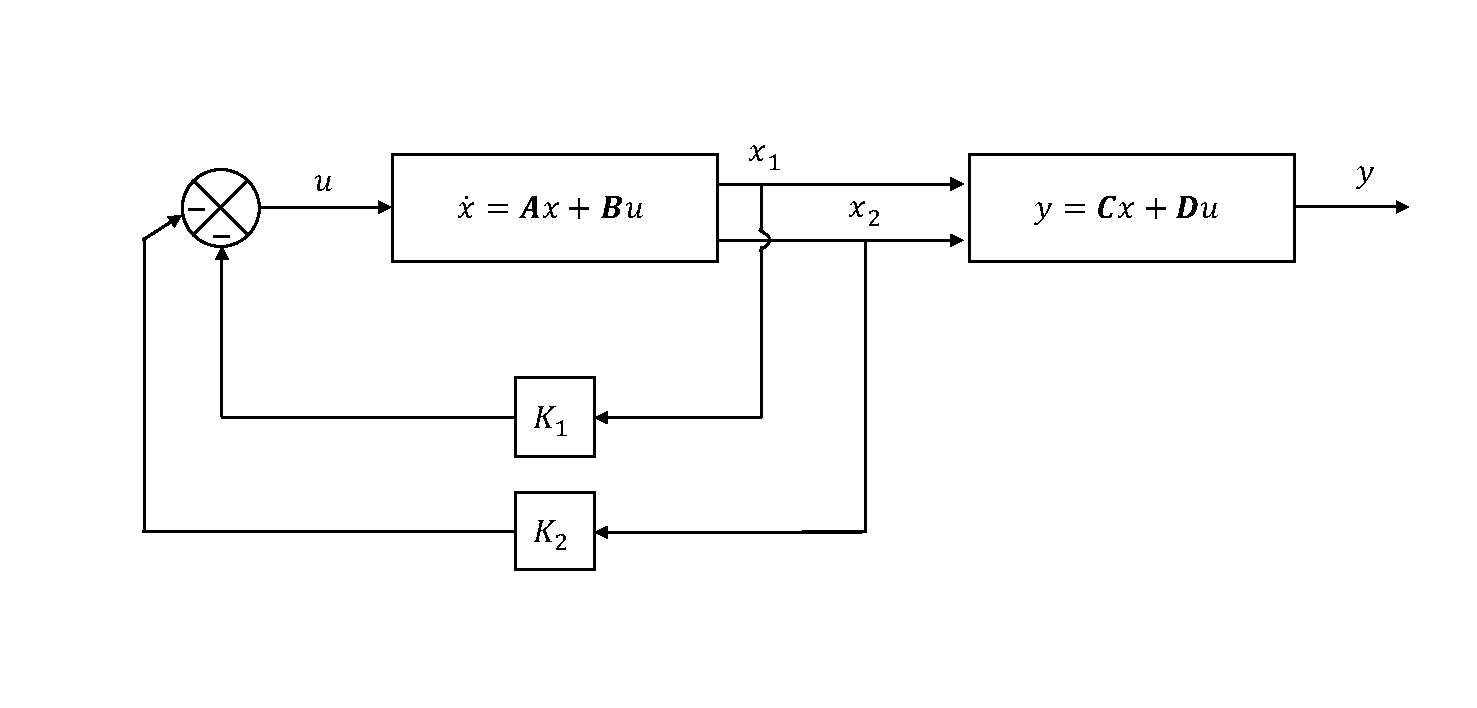
\includegraphics[scale=0.4]{diagrama.pdf}
\caption{LQR controller block diagram}
\label{fig:block_diagram}
\end{figure}

The state space representation \ref{eq:state_space}, \ref{eq:state_space_out} is a controllable canonical form that is important for the LQR controller design. It is desired to keep the actual ZMP, measured and computed by force-torque sensors located in the feet of the humanoid robot, close to its stable reference position as was discussed in previous sections. As the system is a type 0 plant, it is necessary to insert an integrator in order to design a ZMP servo control system (type 1) and remove the steady state error. Therefore, we feed the output signal $y$ (which indicates the real ZMP) back to the input and an integrator in the feedforward path as is shown in Figure \ref{fig:diagrama_int}. Here, $z$ denotes the error between the actual and the reference ZMP, $u$ represents the commanded angle to the system and $u_D$ is the corresponding angle to the reference ZMP ($r$).

\begin{figure}[!hbt]
\centering
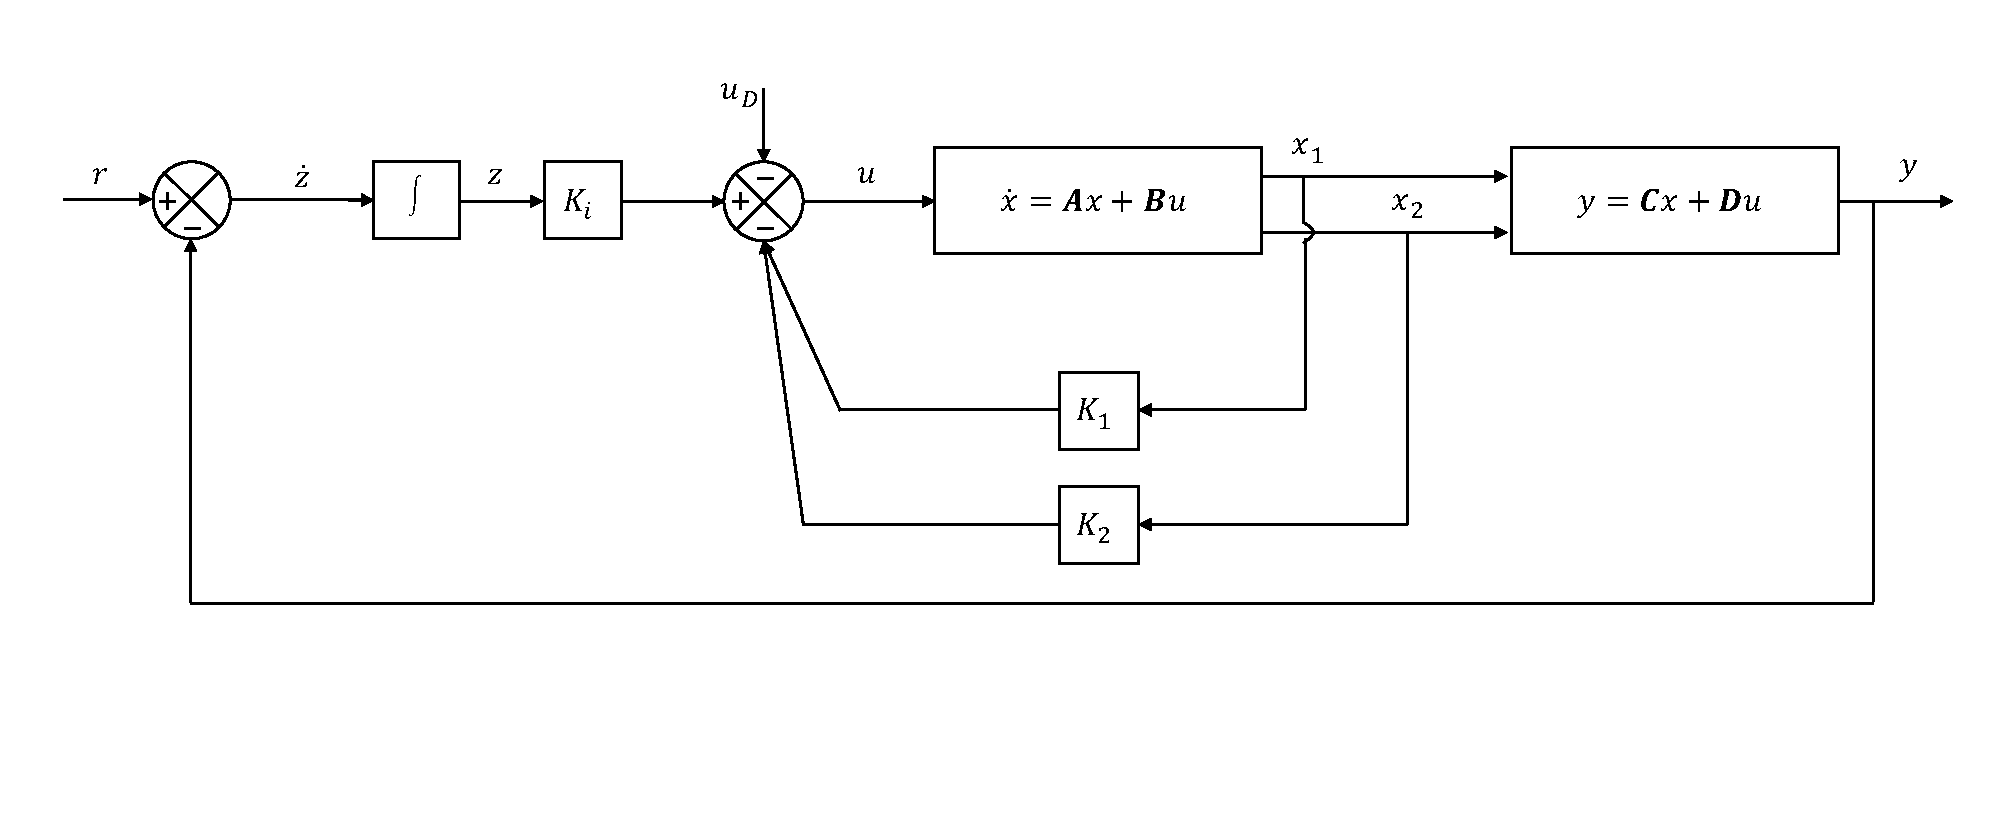
\includegraphics[scale=0.4]{diagrama_int.pdf}
\caption{ZMP LQR control system.}
\label{fig:diagrama_int}
\end{figure}

Thus, referring equations \ref{eq:state_space} and \ref{eq:state_space_out} and Figure \ref{fig:diagrama_int} and considering the actual ZMP position as the output of the system and $r$ as the reference input signal we obtain the equations for the closed loop system as follows:
\begin{equation}
\mathbf{\dot{x}} = \mathbf{A}\textbf{x} + \mathbf{B}u
\end{equation}

\begin{equation}
y = \textbf{C}\textbf{x} + \textbf{D}u
\end{equation}

\begin{equation}
u = - \textbf{K}\textbf{x} + K_i z - K_u u_D
\end{equation}

\begin{equation}
\dot{z} = r - y = r - (\textbf{C}\textbf{x} + \textbf{D}u)
\end{equation}

For the type 1 servo system, the state error equation is given by:
\begin{equation}
\begin{bmatrix}
\dot{\textbf{x}}\\
\dot{z}
\end{bmatrix} = 
\begin{bmatrix}
\textbf{A} & \textbf{0}\\
\textbf{-C} & 0
\end{bmatrix}
\begin{bmatrix}
\textbf{x}\\
z
\end{bmatrix} + 
\begin{bmatrix}
\textbf{B}\\
0
\end{bmatrix}
u
\end{equation}
and the control signal $u$ is given by:
\begin{equation}
u = \begin{bmatrix}
-\textbf{K} & K_i
\end{bmatrix}
\begin{bmatrix}
\textbf{x}\\
z 
\end{bmatrix}
- K_u u_D
\end{equation}

The optimum $K$ matrix is obtained from equations \ref{eq:Kcont} and \ref{eq:Kdisc}.
\begin{equation}
K = R^{-1}B^{T}P \quad (continuous \quad case)
\label{eq:Kcont}
\end{equation}
\begin{equation}
K = (R + B^{T}PB)^{-1}B^{T}PA \quad (discrete \quad case)
\label{eq:Kdisc}
\end{equation}

where $P$ is a positive-definite Hermitian or real symmetric matrix and it is necessary to compute the algebraic Ricatti Equation
\begin{equation}
P \rightarrow A^{T}P+PA-PBR^{-1}B^{T}P+Q = 0 \quad (continuous \quad case)
\end{equation}
\begin{equation}
P \rightarrow A^{T}PA+P-A^{T}PB(R+B^{T}PB)^{-1}B^{T}PA+Q = 0 \quad (discrete \quad case)
\end{equation}


In order to obtain the controller design for further simulations and experiments, the following mechanical parameters of the inverted pendulum (corresponding to Rh-2 humanoid robot) were taken: $m$ = 62.416 kg, $l$=1.03 m, $k$=200. The high stiffness value is due to the rigidity of the pendulum (the leg in this case). If it has a high stiffness, the pendulum will behave as a so rigid link, but if it is lower, the pendulum will be considered as a flexible link and will react in a slower way.

For the optimum response of the control system, it is suggested \textcolor{red}{REFERENCIA?} to take $Q = C^{T}C = \begin{bmatrix}
0.9487 & 0\\
0 & 0
\end{bmatrix}$ and $R = 1 $. 
%%% AÑADIR SOLO SI SE PRUEBA QUE ES MAS RAPIDO %%%%
%But for a faster response of the control, we take $Q = C^{T}C = \begin{bmatrix}
%1000 & 0\\
%0 & 0
%\end{bmatrix}$.  
After the LQR controller was designed, the control gains matrix $K = [12.5527 \quad 4.9178]$ was obtained using a sample time $T = 0.03$ s.












\section{Stabilizer}
Previously it was shown that the dynamics of a humanoid robot can be a single inverted pendulum and how the pendulum maintains a desired position thanks to the controller designed. Now, let us introduce the detailed stabilizer structure (Figure \ref{fig:stabilizer}).

\begin{figure}[!h]
\centering
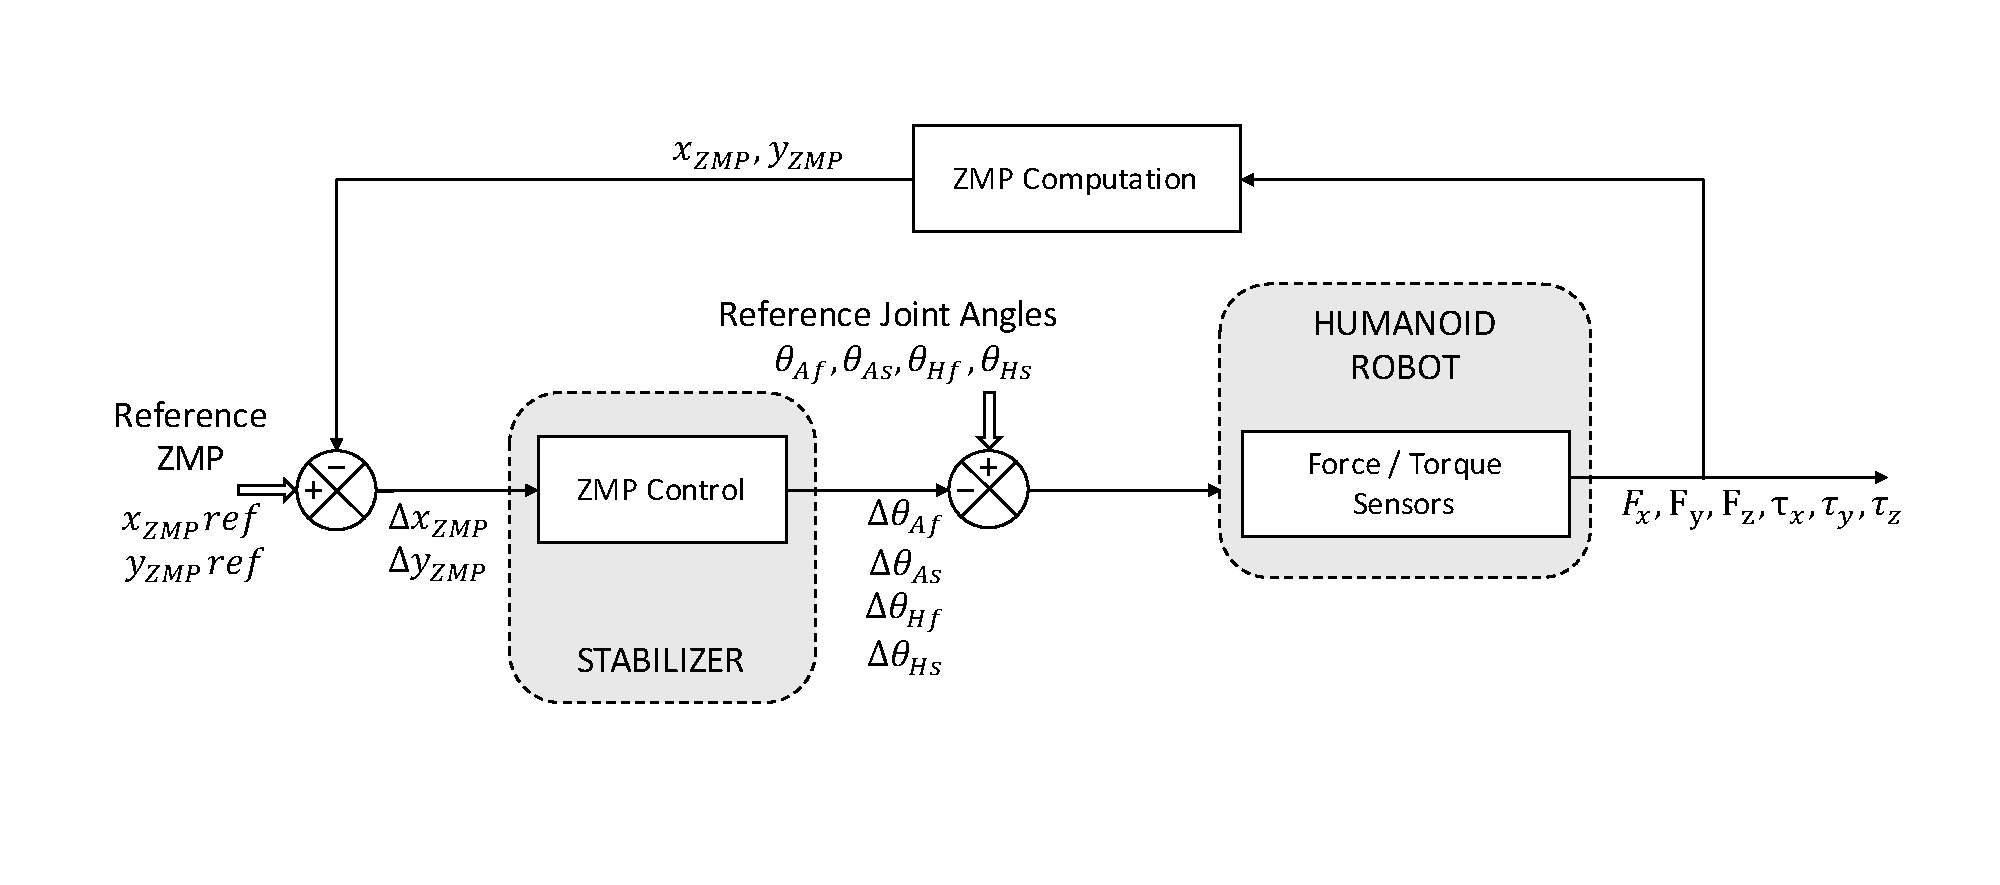
\includegraphics[scale=0.4]{stabilizer.pdf}
\caption{Stabilizer architecture.}
\label{fig:stabilizer}
\end{figure}

The sensorial system of the robot consisting of two six-axis force-torques located at the robot ankles, provides the controller the real distribution of the forces and torques $F_x$, $F_y$, $F_z$, $\tau_x$, $\tau_y$, $\tau_z$ at the contact point of the foot with the ground. After the actual ZMP position $x_{ZMP}$, $y_{ZMP}$ is computed, the ZMP $\Delta x_{ZMP}$, $\Delta y_{ZMP}$ errors can be estimated. These errors are the input data for the Stabilizer and it controls the error in ZMP positioning of the humanoid robot by the motion of the ankle and hip joints.


\section{Control strategies}
Humans are capable of performing numerous dynamical movements in a wide variety of complex and novel environments while robustly rejecting a large spectrum of disturbances. Human movements such as a forward step and rapid arm rotations allow them to maintain overall balance in non-stability situations. Many researchers have studied how humans unwittingly use their body parts to recover balance as a response of external disturbances and make an approach for studying the stability of humanoid robots.

When the humanoid robot is in a stable posture, perturbantions may appear and they can be classified according the direction of action of that perturbations (remember the ZMP areas previously mentioned). All of them can be decomposed in anteroposterior disturbances (sagittal plane) and mediolateral disturbances (frontal plane). Studies of quiet stance have suggested separate postural strategies for balance in both planes depending on the stance position [Day, et al. 1993; Winter, et al. 1996]. There are three main mechanisms that can be applied to regain balance in such planes depending on the level of the disturbance: ankle, hip and step strategies.

The first is the ankle strategy. This strategy is applied in the sagittal plane or anteroposterior disturbances. For low intensity disturbances, the body can be considered as a nearly stiff pendulum, and balance adjustmensts are mainly made in the ankle joint, with the body balancing like a single inverted pendulum (Nashner, 1985). 

In the hip strategy, the resulting motion is mainly applied to the hip joints (Horak, et al. 1990). It can be applied independently or in combination of the ankle strategy. The hip joint movement is triggered when the external disturbance increases and the ankle strategy is not enough to keep balance. The hip strategy, same as ankle one, acts in the anteroposterior direction.

The last one is the step strategy. When these postural corrections become insufficient, the base of support must be adjusted (Carr, et al. 1987; Horak, et al. 1990). The modification of the support base leads new balance stability limits.

Figure (¿?) sumarizes this three strategies and Figure \ref{fig:strategies} shows the levels for strategy triggering. These limits are not fixed and they depend of the humanoid design as the sole surface or the height of the whole body, environmental conditions, i. e, standing in a flat surface has different strategy limits than in a narrow surface.

\begin{figure}[!htbp]
\centering
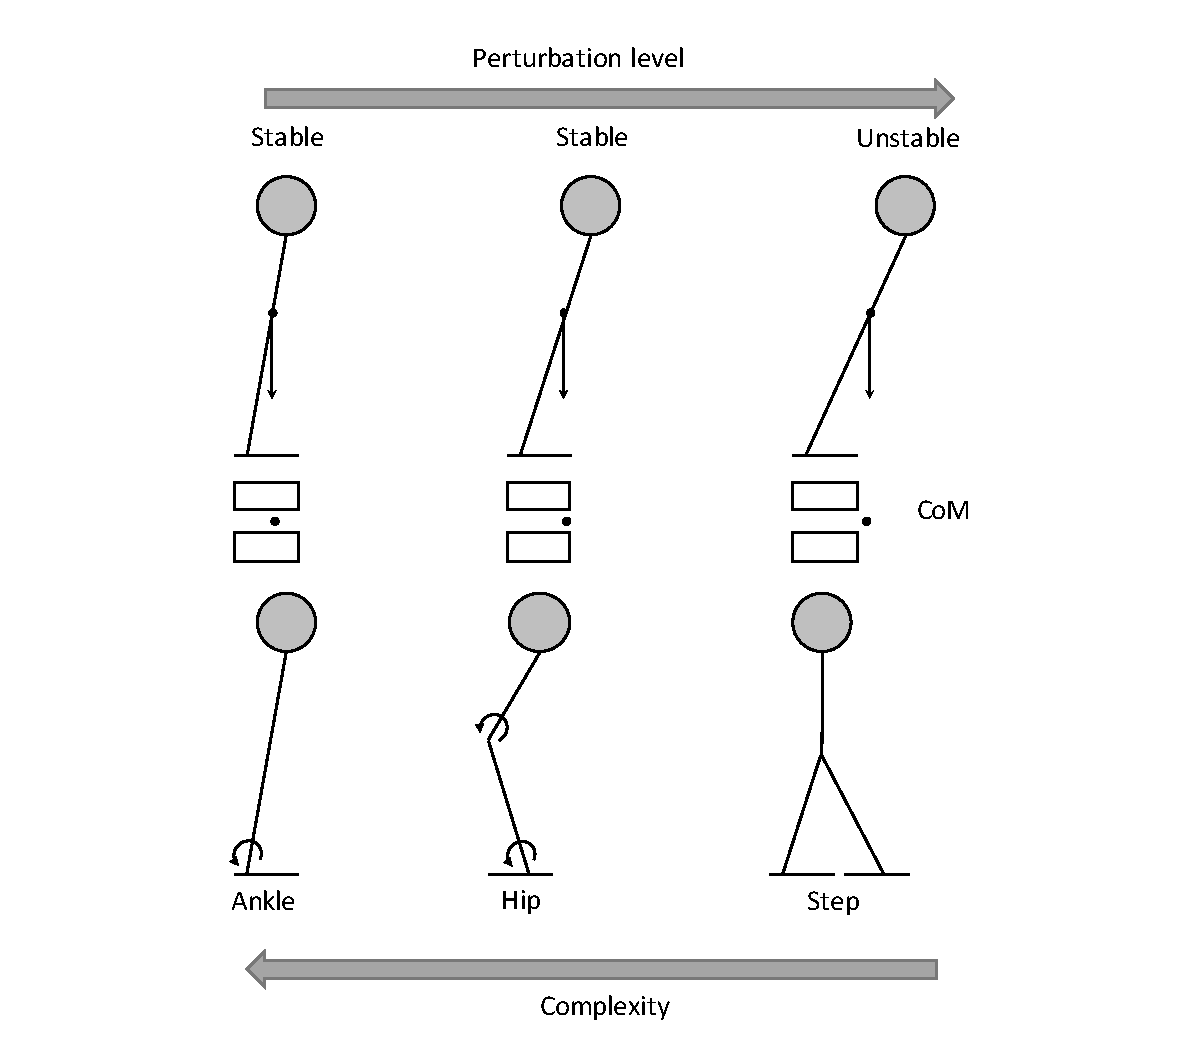
\includegraphics[scale=0.5]{strategies.pdf}
\caption{Recovery strategies.} \label{fig:strategies}
\end{figure}

In the mediolateral direction or frontal plane, the disturbances are compensated by the lateral movement of the hip joint in the case of upright stance. Double support in frontal plane, means there are two support points and a pendulum can not be considered. Both legs and the trunk of the robot make a parallelogram with the ground (see Figure \ref{fig:piernas} (a)). If a disturbance appears, and the hips maintain their perpendicular angles to the body, the feet will begin to loose contact with the ground as shown in Figure \ref{fig:piernas} (b). Then, to maintain stability, the angles of the parallelogram must keep on their relationship without loosing contact between feet and the ground, and the motion is applied to ankle and hip joints (Figure \ref{fig:piernas} (c)). 


\begin{figure}[!htbp]
\centering
\subfigure[]{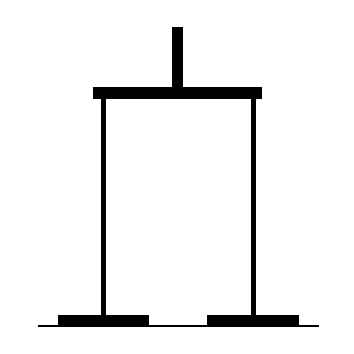
\includegraphics[width=40mm]{piernas1.pdf}}
\subfigure[]{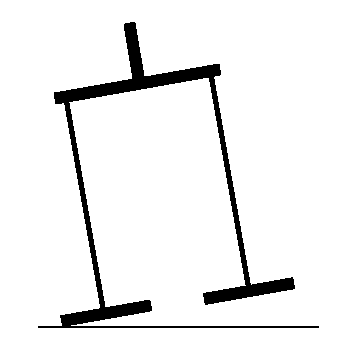
\includegraphics[width=40mm]{piernas2.pdf}}
\subfigure[]{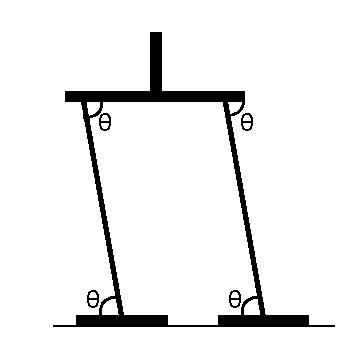
\includegraphics[width=40mm]{piernas3.pdf}}
\caption{Influence of hip and ankle angles in the frontal plane stability.} \label{fig:piernas}
\end{figure}



